\documentclass[border=5mm]{standalone}
\usepackage{tikz}
\usepackage{tikz-qtree}

\begin{document}
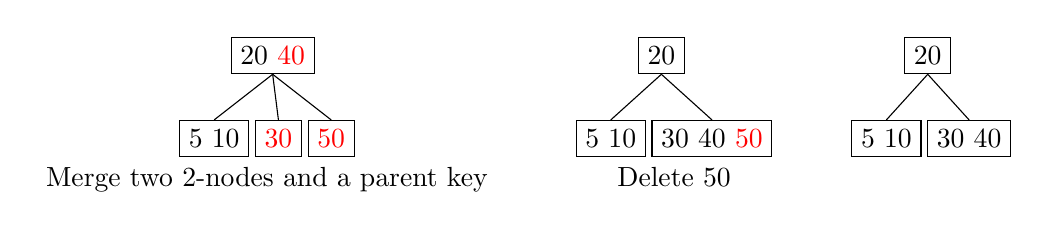
\begin{tikzpicture}[every tree node/.style={align=center}]
    \matrix[row sep=1cm, column sep=1cm] {
    \Tree
    [.\node[draw, rectangle]{20 \textcolor{red}{40}};
    [.\node[draw, rectangle]{5 10}; ]
    [.\node[draw, rectangle]{\textcolor{red}{30}}; ]
    [.\node[draw, rectangle]{\textcolor{red}{50}};    ]
    ];
    \node[below] at (current bounding box.south) {Merge two 2-nodes and a parent key};
    &
    \Tree
    [.\node[draw, rectangle]{20};
    [.\node[draw, rectangle]{5 10}; ]
    [.\node[draw, rectangle]{30 40 \textcolor{red}{50}}; ]
    ];  
    \node[below] at (current bounding box.south) {Delete 50};
    &
    \Tree
    [.\node[draw, rectangle]{20};
    [.\node[draw, rectangle]{5 10}; ]
    [.\node[draw, rectangle]{30 40}; ]
    ];  \\
    };

\end{tikzpicture}
\end{document}
